\chapter{Analiza wydajnościowa}

Poniższy rozdział opisuje przeprowadzane testy na wszystkich wersjach systemu.
Każda wersja została poddana jednakowej procedurze testowej.
Następnie wyniki zostały poddane analizie porównawczej i zostały wyciągnięte z nich wnioski.

\section{Testowa konfiguracja środowiska}

Testy zostały przeprowadzone na komputerze stacjonarnym z następującą konfiguracją sprzętową:
\begin{itemize}
    \item \textbf{procesor}: Intel Core i7-3770 (4-rdzeniowy/8-wątkowy taktowany zegarem 3,4 GHz),
    \item \textbf{pamięć operacyjna}: 8 GB,
    \item \textbf{dysk twardy} o pojemności 500 GB (7200 RPM, SATA 6 Gb/s),
    \item \textbf{system operacyjny}: Microsoft Windows 10 Professional (x64) Build 17134.345
\end{itemize}

Środowisko systemu zostało utworzone z wykorzystaniem narzędzia do konteneryzacji aplikacji jakim jest Docker.
Na systemie Windows wymaga to dodatkowo zainstalowania \textit{Oracle VirtualBox} w celu utworzenia maszyny wirtualnej ze specjalną dystrybucją systemu Linux -- \textit{Tiny Core Linux}.
To wszystko jest dostarczane wraz z pakietem \textit{Docker Toolbox for Windows}.
Na takiej maszynie wirtualnej następnie są uruchamiane kontenery Dockera.

W ramach testów powstały środowiska dla każdej z trzech wersji systemu.
Ze względu na ograniczenia sprzętowe, spowodowane niedostateczną ilością pamięci operacyjnej, niemożliwe było utworzenie wirtualnego klastra bazodanowego dla baz Apache Cassandra i MongoDB, dlatego też testowany system współpracował z pojedynczą instancją każdej z baz.

\section{Narzędzie symulujące obciążenie}

Głównym narzędziem do testowania był program Apache JMeter 5.
Jest to aplikacja open-source, napisana w języku Java i zaprojektowana do przeprowadzania testów wydajnościowych i~obciążeniowych wielu różnych systemów.
Pozwala ona symulować realny ruch użytkowników na wiele sposobów.
Zalety przemawiające za użyciem tego narzędzia to:
\begin{itemize}
    \item wieloplatformowość pozwalająca na uruchomienie go w niemal każdym środowisku,
    \item funkcjonalny interfejs użytkownika,
    \item możliwość tworzenia skomplikowanych scenariuszy testowych,
    \item możliwość uruchamiania stworzonych scenariuszy zdalnie z wielu maszyn równocześnie,
    \item spore możliwości gromadzenia i analizy statystyk.
\end{itemize}

\section{Porównywane metryki}

%% Jak szybko baza pada
%% Zmiana czasu odpowiedzi w zależności od obciążenia
%% Przepustowość

Podczas testów zostały zbadane następujące metryki:
\begin{itemize}
    \item \textbf{Przepustowość systemu}, która rozumiana jest jako liczba żądań i odpowiedzi na nie, których jest w stanie udzielić serwer w jednostce czasu (na sekundę).
    \item \textbf{Czas odpowiedzi} aplikacji na żądania.
\end{itemize}

Metryki te były mierzone w zależności od symulowanego obciążenia.
Dzięki temu udało się zbadać wpływ wybranego modelu i bazy danych na nie.

\section{Scenariusze testowe}

Wydajność, oprócz niezawodności, jest jednym z głównych czynników decydujących o przydatności bazy danych w warunkach produkcyjnych. 
Wiele baz danych typu NoSQL szczyci się bardzo wysokim poziomem niezawodności oraz wydajności, dlatego podczas tworzenia scenariuszy testowych skupiłem się na dwóch podstawowych operacjach -- odczytu i zapisu -- w kontekście różnych obciążeń.

\subsection{Testy operacji zapisu} \label{sec:zapisScenariusz}

Bezawaryjność i szybkość zapisu danych do bazy w aplikacjach internetowych ma duże znaczenie, zwłaszcza w systemie, w którym często są zapisywane pliki.
W takim przypadku zapis może być nawet bardziej kosztowny czasowo niż operacja odczytu danych.
W przy zapisie często też trzeba zadbać o transakcyjność operacji.
MongoDB w używanej w stworzonym systemie wersji zapewnia wsparcie dla transakcji między wieloma kolekcjami.
System korzysta z możliwości jaką daje ta baza i operacje zapisu obejmujące wiele kolekcji posiadają kontekst transakcyjny.
Trochę inaczej wygląda sytuacji w przypadku bazy danych Apache Cassandra -- operacje zapisu są atomowe na poziomie zapisu pojedynczego wiersza.
Oznacza to, że system musi sam zadbać o~spójność zapisu i wycofać zmiany jeśli cokolwiek pójdzie nie tak.

Do testowania operacji zapisu w każdej wersji systemu był użyty scenariusz obejmujący następujące kroki użytkownika:
\begin{enumerate}
    \item Zalogowanie się do systemu.
    \item Utworzenie nowego projektu.
    \item W pętli powtarzającej się 10-krotnie użytkownik:
    \begin{enumerate}
        \item tworzył nowe zadanie,
        \item dodawał do niego 10 nowych plików do zadania.
    \end{enumerate}
\end{enumerate}
Przed każdym testem baza danych była czyszczona i generowana była odpowiednia liczba użytkowników, a całe środowisko restartowane.

\subsection{Testy operacji odczytu} \label{sec:readTestScenario}

Od szybkości operacji odczytu danych z bazy zależy ogólne wrażenie szybkości działania użytkowanego systemu.
Duże opóźnienia mogą spotęgować złe warażenia z poruszania się po systemie i przypiąć mu łatkę ociężałego i powolnego.

Do testowania operacji odczytu w każdej wersji systemu był użyty scenariusz obejmujący następujące kroki użytkownika:
\begin{enumerate}
    \item Zalogowanie się do systemu.
    \item Pobranie listy projektów, w których uczestniczy zalogowany użytkownik.
    \item Dla każdego projektu pobranie listy zadań do niego przypisanych, do których ma dostęp użytkownik.
    \item Dla każdego pobranego zadania pobranie listy plików do niego przypisanych.
    \item Pobranie najnowszej wersji każdego pliku zwróconego w poprzednim kroku.
\end{enumerate}
Przed każdym testem baza danych była uzupełniona odpowiednią liczbą użytkowników.
Dla każdego użytkownika był generowany jeden projekt z 10 zadaniami, a każde zadanie posiadało 10 plików.
Po pojedynczym teście całe środowisko było restartowane.

\section{Wyniki testów i ich omówienie}

\subsection{Operacja zapisu danych}

Testy operacji zapisu danych zostały przeprowadzone za pomocą symulacji 100 użytkowników odtwarzających scenariusz opisany w sekcji \ref{sec:zapisScenariusz}.
Liczba wirtualnych użytkowników przy zadanym scenariuszu przełożyła się na 11200 zapytań HTTP do serwera w trakcie testu.
Próby symulacji większego obciążenia dla pojedynczej instancji systemu na posiadanej platformie testowej powodowały, że stawał się on wąskim gardłem dla testów.
Serwer aplikacyjny był wtedy obciążony w 100\% i nie nadążał z szybkim przyjmowaniem i przetwarzaniem zapytań, które były kolejkowane, zawyżając w znacznym stopniu mierzone metryki, a w najgorszym przypadku serwer odrzucał próby połączenia.

Tabela \ref{tab:resultsSaveOp} przedstawia podsumowanie wyników przeprowadzonych testów.
Widoczna jest znaczna przewaga modelu hybrydowego. 
W modelu tym podczas dodawania nowego pliku do systemu tworzone są wpisy do dwóch tabel: jeden do tabeli \textit{file\_metadata} w PostgreSQL, drugi do tabeli \textit{version} w Cassandrze.
Co ważne nie jest wymagane ponowne zliczanie liczby plików w zadaniu w celu zaktualizowania statystyk zadania i projektu, co ma miejsce w przypadku pozostałych dwóch modeli danych.
Dzięki normalizacji danych i braku potrzeby przeliczania zagregowanych informacji liczba operacji zapisu do bazy danych jest mniejsza, w związku z~tym całkowity czas odpowiedzi również jest mniejszy.
W próbie testowej lwią część stanowią operacje dodania nowego pliku do zadania. 
Operacja ta obejmuje w dużej mierze zapis do bazy Apache Cassandra, który jest operacją szybszą niż zapis w bazie PostgreSQL co skutkuje szybszą odpowiedzią na żądanie HTTP. 

\begin{table}[!ht]
\centering
\begin{tabular}{|c|c|c|c|c|c|c|c|}
\hline
\multirow{2}{*}{Model danych} & \multicolumn{6}{c|}{Czas odpowiedzi (ms)} & \multirow{2}{*}{\begin{tabular}[c]{@{}c@{}}Przepustowość\\ (zapytania/s)\end{tabular}} \\ \cline{2-7}
 & Średni & Min & Max & 90 per & 95 per & 99 per &  \\ \hline
Apache Cassandra & 2818.62 & 169 & 14609 & 3969 & 4628.90 & 8293.25 & 35.06 \\ \hline
MongoDB & 2170.88 & 18 & 9420 & 3754 & 4495.95 & 7288.81 & 44.91 \\ \hline
\begin{tabular}[c]{@{}c@{}}Apache Cassandra\\ + PostgreSQL\end{tabular} & 1581.61 & 11 & 6010 & 2609 & 3027.90 & 3958.98 & 61.12 \\ \hline
\end{tabular}
\caption{Wyniki testów zapisu dla 100 równolegle pracujących użytkowników}
\label{tab:resultsSaveOp}
\end{table}

Warte odnotowania jest, że pomimo lepszej ogólnej wydajności dla zadanego scenariusza testowego system z modelem hybrydowym uzyskiwał znacznie dłuższe czasy odpowiedzi na żądania utworzenia nowego zadania.
Widać to na rysunku \ref{fig:hybridSaveTaskDistribution} przedstawiającym wykres z rozkładem żądań utworzenia nowego zadania w dziedzinie czasu odpowiedzi, gdzie jest on znacznie szerszy i~bardziej płaski niż w przypadku pozostałych dwóch wersji systemu, których analogiczne rozkłady zostały przedstawione kolejno na rysunkach \ref{fig:cassandraSaveTaskDistribution} i \ref{fig:mongoSaveTaskDistribution}.
Na tym tle najlepiej wyszedł system z bazą MongoDB, gdzie połowa żądań utworzenia nowego zadania uplasowała się w czasie odpowiedzi poniżej 160 ms, a maksymalny czas nie wyniósł więcej niż 1,6 s.

\begin{figure}[!ht]
\centering
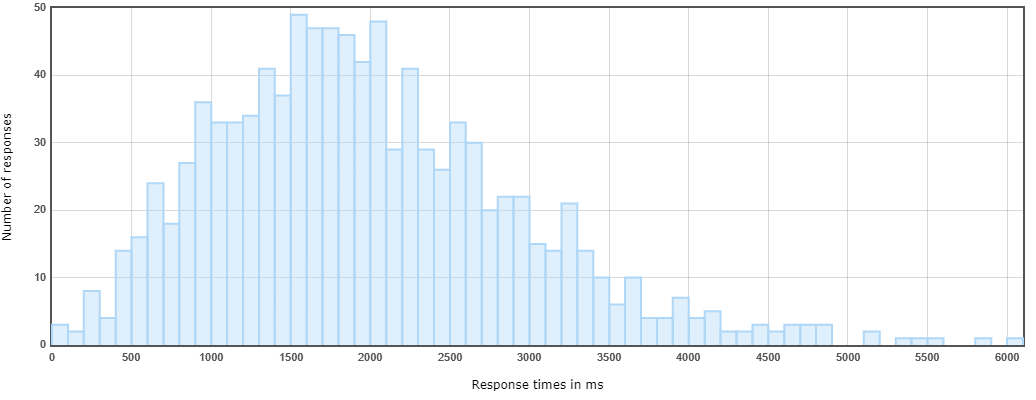
\includegraphics[width=\textwidth]{figures/flotResponseTimeDistribution_hybrid_save.png}
\caption{Rozkład liczby żądań utworzenia nowego zadania w dziedzinie czasu odpowiedzi dla modelu hybrydowego}
\label{fig:hybridSaveTaskDistribution}
\end{figure}

\begin{figure}[!ht]
\centering
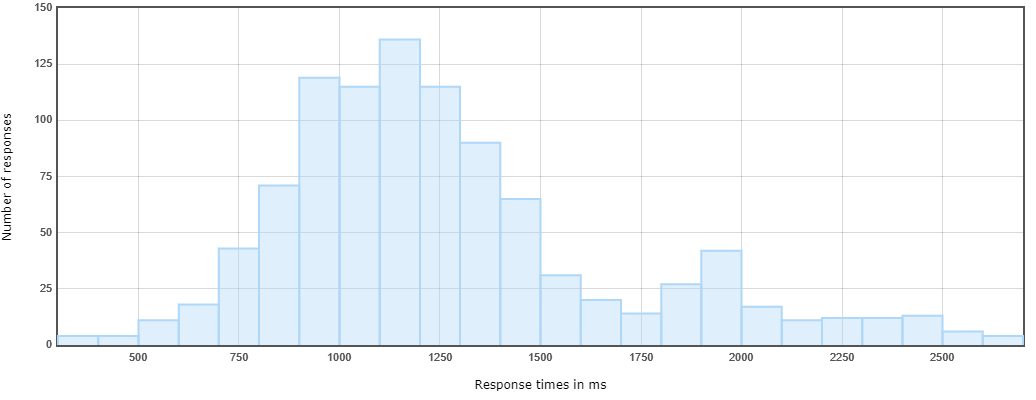
\includegraphics[width=\textwidth]{figures/flotResponseTimeDistribution_cass_save.png}
\caption{Rozkład liczby żądań utworzenia nowego zadania w dziedzinie czasu odpowiedzi dla modelu Apache Cassandra}
\label{fig:cassandraSaveTaskDistribution}
\end{figure}

\begin{figure}[!ht]
\centering
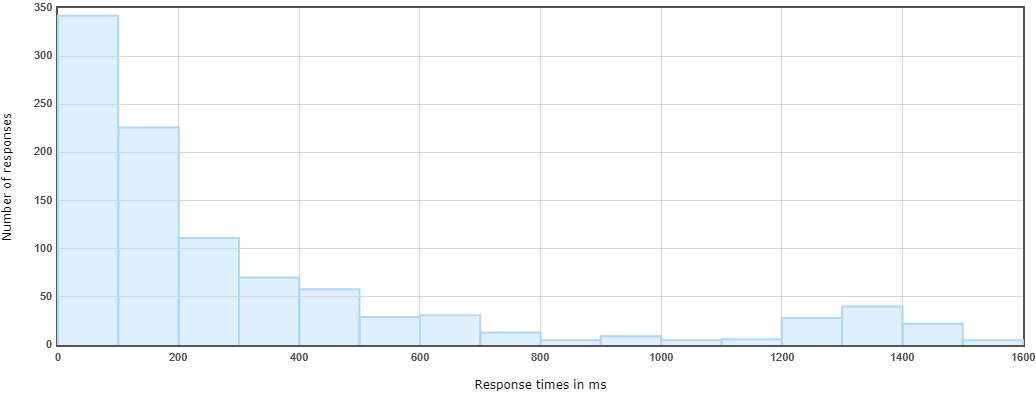
\includegraphics[width=\textwidth]{figures/flotResponseTimeDistribution_mongo_save.png}
\caption{Rozkład liczby żądań utworzenia nowego zadania w dziedzinie czasu odpowiedzi dla modelu MongoDB}
\label{fig:mongoSaveTaskDistribution}
\end{figure}

\subsection{Operacja odczytu danych}

Testy operacji odczytu danych zostały przeprowadzone z symulacją 1000 użytkowników równolegle odtwarzających scenariusz opisany w sekcji \ref{sec:readTestScenario} dla systemów korzystających wyłącznie z baz Apache Cassandra i MongoDB.
To przełożyło się na sumaryczną liczbę zapytań do serwera aplikacyjnego równą 213000.
Próby symulacji dla większej ilości wirtualnych użytkowników powodowały, że czas odpowiedzi wzrastał, a rzeczywista przepustowość nie ulegała zmianom.
Tabela \ref{tab:resultsReadOp} przedstawia podsumowanie wyników.
System korzystający wyłącznie z Cassandry osiągną znacznie lepsze rezultaty niż system korzystający z MongoDB.
Widać to było również po czasie potrzebnym na ukończenie scenariusz testowego, odpowiednio ok. 13 i 22 minuty.
Dzięki bardzo szybkim odczytom z Cassandry system był w stanie obsłużyć o 63\% więcej żądań na sekundę, co jest wynikiem imponującym.

\begin{table}[!ht]
\centering
\begin{tabular}{|c|c|c|c|c|c|c|c|}
\hline
\multirow{2}{*}{Model danych} & \multicolumn{6}{c|}{Czas odpowiedzi (ms)} & \multirow{2}{*}{\begin{tabular}[c]{@{}c@{}}Przepustowość\\ (zapytania/s)\end{tabular}} \\ \cline{2-7}
 & Średni & Min & Max & 90 per & 95 per & 99 per &  \\ \hline
Apache Cassandra & 3732,41 & 17 & 40871 & 3331 & 3590 & 3739 & 266,69 \\ \hline
MongoDB & 6080,41 & 8 & 124733 & 5888 & 6524,95 & 9127 & 163,45 \\ \hline
\end{tabular}
\caption{Wyniki testów odczytu danych dla 1000 równolegle pracujących użytkowników}
\label{tab:resultsReadOp}
\end{table}

Dla systemu z hybrydowym modelem danych nie udało się przeprowadzić do końca testów z 1000 użytkowników, ponieważ duża liczba zapytań powodowała bardzo szybkie wyczerpywanie się puli połączeń do bazy PostgreSQL i po 30 sekundach oczekiwania na wolne połączenie aplikacja odpowiadała błędem. 
Wątek, symulujący pracę użytkownika, nie mógł kontynuować scenariusz testowego w momencie otrzymania błędnej odpowiedzi i sumaryczna liczba zapytań była znacznie niższa.
Dopiero obniżenie liczby użytkowników do 100 pozwalało na ukończenie testu bez otrzymywania błędów w trakcie jego trwania.

Tabela \ref{tab:resultsRead100} przedstawia wyniki testu dla 100 równolegle pracujących użytkowników w systemie z hybrydowym modelem danych.
Dla porównania przetestowane zostały również pozostałe dwie wersje systemu i wyniki zostały umieszczone w tej samej tabeli.
Możemy z niej odczytać, że najwolniejszą wersją systemu jest ta z dwiema bazami danych.
Była w stanie obsłużyć o~ok.~28\% mniej żądań niż pozostałe dwie wersje i uzyskiwała średnio o ok. 40\% wolniejsze czasy odpowiedzi.

\begin{table}[!ht]
\centering
\begin{tabular}{|c|c|c|c|c|c|c|c|}
\hline
\multirow{2}{*}{Model danych} & \multicolumn{6}{c|}{Czas odpowiedzi (ms)} & \multirow{2}{*}{\begin{tabular}[c]{@{}c@{}}Przepustowość\\ (zapytania/s)\end{tabular}} \\ \cline{2-7}
 & Średni & Min & Max & 90 per & 95 per & 99 per &  \\ \hline
Apache Cassandra & 651,19 & 17 & 3090 & 974 & 1096 & 1286 & 146,49 \\ \hline
MongoDB & 635.89 & 17 & 6212 & 874 & 1055 & 1511,99 & 149,65 \\ \hline
\begin{tabular}[c]{@{}c@{}}Apache Cassandra\\ + PostgreSQL\end{tabular} & 903,96 & 16 & 39557 & 1112 & 1296,95 & 1743,99 & 106,63 \\ \hline
\end{tabular}
\caption{Wyniki testów odczytu danych dla 100 równolegle pracujących użytkowników}
\label{tab:resultsRead100}
\end{table}

Jedną z przyczyn słabych wyników modelu hybrydowego były duże czasy odpowiedzi na żądania pobrania informacji o projektach w jakich uczestniczy użytkownik i informacji o samym projekcie.
Widać to na rysunku \ref{fig:hybridReadResponseTimePercentiles} przedstawiającym wykres czasów odpowiedzi na poszczególne kategorie zapytań w rozkładzie na centyle.
Można z niego odczytać, że 90\% próbek zapytań z~tej kategorii miało czasy odpowiedzi większe niż 4,5 sekundy w kontraście do próbek z pozostały kategorii, które czas odpowiedzi większy niż 5 sekund miały dla ostatnich 8 centyli.
Wynika to z tego, że operacja pobrania listy projektów użytkownika wymaga 3 operacji złączenia tabel, kolejno:
\begin{enumerate}
    \item tabeli \textit{project} z \textit{user}, aby wyszukać projekty, których jest administratorem,
    \item tabeli \textit{project} z \textit{task}, 
    \item tabeli \textit{task} z \textit{user}, aby wyszukać zadania, w których uczestniczy i na podstawie tych zadań pobrać projekty.
\end{enumerate}
Pozostałe operacje zawarte w teście są porównywalnie szybkie do odpowiadającym ich zapytań w pozostałych dwóch systemach.

\begin{figure}[!ht]
\centering
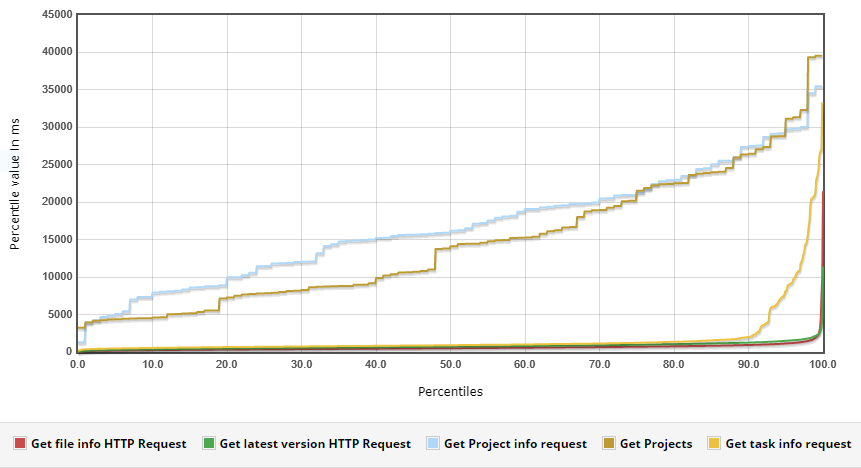
\includegraphics[width=\textwidth]{figures/wykres.PNG}
\caption{Rozkładu centyli czasów odpowiedzi poszczególnych rodzajów żądań testu systemu z modelem hybrydowym}
\label{fig:hybridReadResponseTimePercentiles}
\end{figure}
